\documentclass{article}

\usepackage{neurips_2026}

\usepackage[utf8]{inputenc}
\usepackage[T1]{fontenc}
\usepackage{lmodern}
\usepackage{hyperref}
\usepackage{url}
\usepackage{booktabs}
\usepackage{amsfonts}
\usepackage{amsmath}
\usepackage{amssymb}
\usepackage{amsthm}
\usepackage{nicefrac}
\usepackage{microtype}
\usepackage{xcolor}
\usepackage{colortbl}
\usepackage{graphicx}
\usepackage{subcaption}
\usepackage{multirow}
\usepackage{algorithm}
\usepackage{algpseudocode}
\usepackage{tablefootnote}
\usepackage{enumitem}
\usepackage{tikz}
\usetikzlibrary{shapes,arrows,positioning,fit,calc}
\usepackage{wrapfig}

% ---------- Custom colors and commands ----------
\definecolor{improve}{RGB}{0,128,0}
\definecolor{decline}{RGB}{200,0,0}
\definecolor{easycolor}{RGB}{76,175,80}
\definecolor{medcolor}{RGB}{255,152,0}
\definecolor{hardcolor}{RGB}{244,67,54}
\definecolor{nothinkblue}{RGB}{31,119,180}
\definecolor{thinkorange}{RGB}{255,127,14}

\newcommand{\up}[1]{\textcolor{improve}{\textbf{+#1}}}
\newcommand{\down}[1]{\textcolor{decline}{\textbf{#1}}}
\newcommand{\ci}[2]{\scriptsize[#1,\,#2]}
\DeclareMathOperator*{\argmax}{arg\,max}
\DeclareMathOperator*{\argmin}{arg\,min}
\newcommand{\method}{\textsc{TOWN}}
\newcommand{\fullmethod}{Think Only When Needed}
\newcommand{\thinkingtax}{\emph{thinking tax}}

% ---------- Theorem environments ----------
\newtheorem{theorem}{Theorem}
\newtheorem{proposition}{Proposition}
\newtheorem{corollary}{Corollary}
\newtheorem{definition}{Definition}
\newtheorem{assumption}{Assumption}
\theoremstyle{remark}
\newtheorem{remark}{Remark}
\newtheorem{observation}{Observation}

% ---------- Figure path ----------
\graphicspath{{../results/paper_figures/}}

% ---------- Title ----------
\title{The Thinking Tax: When Chain-of-Thought Costs More Than It Saves}

\author{
  Anonymous Author(s)
}

\begin{document}

\maketitle

% ============================================================================
% ABSTRACT
% ============================================================================
\begin{abstract}
Chain-of-thought (CoT) reasoning is widely believed to improve LLM accuracy by allowing models to ``think longer.''
We show this improvement requires a \emph{crossover budget} far higher than commonly assumed: below this task- and model-specific threshold, thinking mode \emph{underperforms} non-thinking mode by up to 69.5 percentage points---a phenomenon we call the \emph{thinking tax}.
On GSM8K and MATH-500 with Qwen-family models (8B, 9B, 27B), non-thinking outperforms thinking at every budget below the crossover; the mechanism is truncation waste---at budget 256, 98.6\% of thinking responses are cut off before reaching an answer.
We formalize this via a truncation-waste decomposition that, given empirically measured completion rates and accuracy gaps, yields closed-form estimates of thinking-mode accuracy and the crossover from chain-length statistics, consistent with measurements across both benchmarks.
The tax \emph{worsens with model size}---2.7--2.9$\times$ larger for 9B/27B vs.\ 8B---as longer chains demand larger budgets.
Building on these insights, we propose \method{} (\fullmethod{}), a training-free cascade that routes only budget-exhausting queries to extended thinking.
\method{} achieves \textbf{90.9\%} at 199 avg tokens (+25.7\,pp over think@512 at 2.3$\times$ fewer tokens), with Pareto improvement guarantees under a verifiable net-recovery condition.
Our results suggest the key question is not \emph{how long} to think, but \emph{whether} to think at all.
\end{abstract}

% ============================================================================
\section{Introduction}
\label{sec:intro}
% ============================================================================

% introduction_compact.tex — Compressed introduction for 9-page version

\begin{figure}[t]
    \centering
    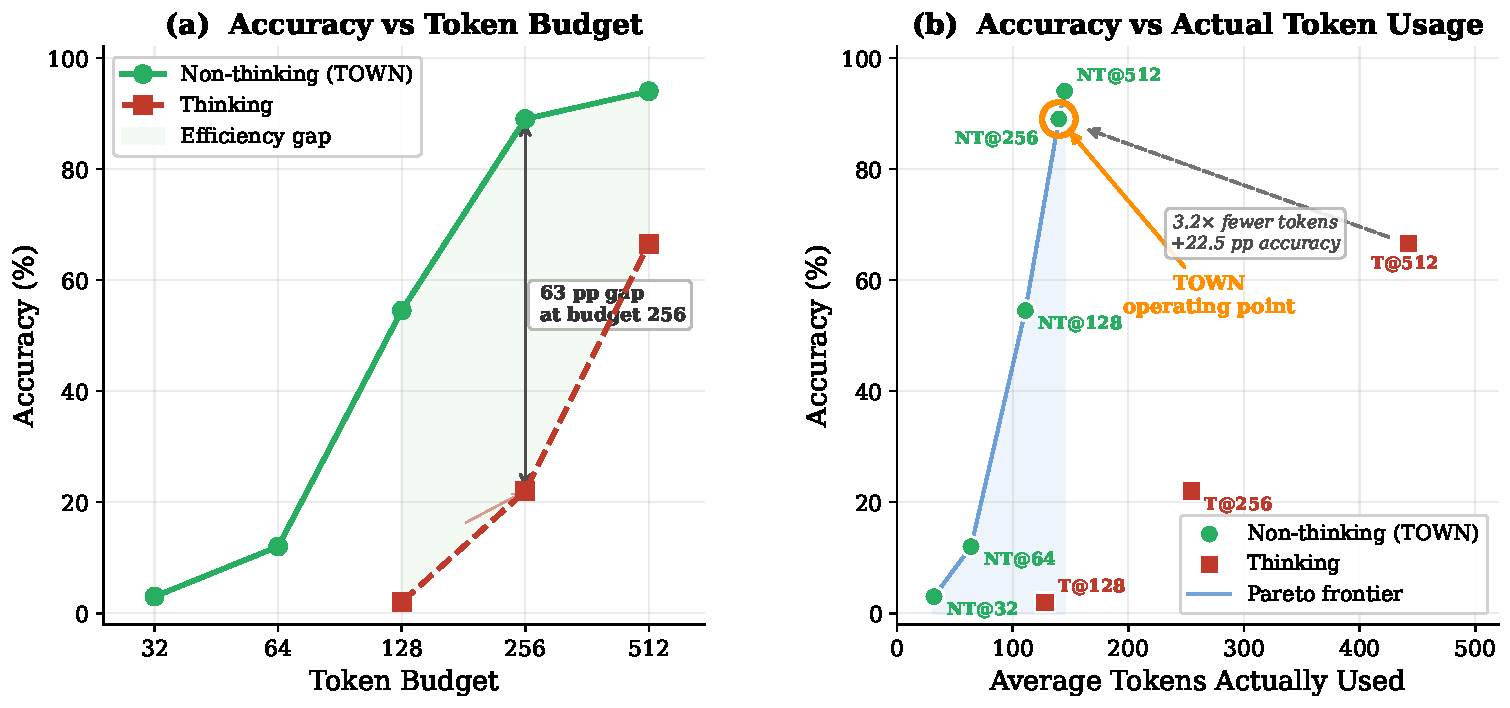
\includegraphics[width=\linewidth]{fig_nothink_vs_thinking.pdf}
    \caption{\textbf{The Thinking Tax.}
    Non-thinking mode (blue) outperforms thinking mode (orange) at \emph{every} matched token budget on GSM8K (Qwen3-8B), by up to \textbf{+22.3\,pp} at 3.2$\times$ fewer tokens.}
    \label{fig:nothink-vs-thinking}
\end{figure}

More thinking tokens, more accuracy---this is the implicit contract of chain-of-thought (CoT) reasoning~\citep{wei2022chain}, now operationalized in systems like DeepSeek-R1~\citep{deepseekr1} and Qwen3~\citep{qwen3_2025}.
We show this contract is broken: below a task- and model-specific token budget, thinking mode \emph{degrades} accuracy by up to 69.5 percentage points, and the penalty \textbf{worsens} with model scale.
The crossover budget where thinking catches up is far higher than commonly assumed.

\paragraph{The thinking tax.}
Through experiments on GSM8K, MATH-500, and five BIG-Bench Hard subtasks with three Qwen-family model sizes (8B, 9B, 27B), we find that \textbf{below the crossover budget, non-thinking mode outperforms thinking mode at every tested budget, often by a wide margin} (Figure~\ref{fig:nothink-vs-thinking}).
The crossover occurs at ${\sim}$2048 tokens on GSM8K; on MATH-500, it shifts further right, beyond 2048 tokens.
As Figure~\ref{fig:nothink-vs-thinking} illustrates, non-thinking@256 outperforms thinking@512 by +22.3\,pp at 3.2$\times$ fewer tokens; on MATH-500, the gap exceeds \textbf{41.8\,pp} at budget 1024.
The root cause is \emph{truncation waste}: thinking mode's verbose chains are truncated before reaching the answer.
The tax \emph{worsens with model size}---2.9$\times$ and 2.7$\times$ larger for 9B and 27B vs.\ 8B---as larger models generate longer chains.

\paragraph{Natural stopping as free confidence signal.}
When thinking mode completes its chain before exhausting the budget (a \emph{natural stop}), accuracy is 96.3\%---nearly perfect---vs.\ 46.6\% for truncated samples.
This binary, endogenous signal requires no logit access and enables zero-cost routing between modes.

\paragraph{Contributions.}
\begin{enumerate}[nosep,leftmargin=*]
    \item \textbf{The Thinking Tax} (\S\ref{sec:thinking-tax}): non-thinking outperforms thinking at all budgets below a crossover (${\sim}$2048 on GSM8K; ${>}$2048 on MATH-500; 1024--2048 on BBH), with the gap \emph{worsening} with model size (2.7--2.9$\times$ for 9B/27B vs.\ 8B) and task difficulty. The truncation mechanism also replicates on DeepSeek-R1-Distill-Llama-8B (Appendix~\ref{app:deepseek}), consistent with the tax transferring across open reasoning models.
    \item \textbf{Truncation-Waste Decomposition} (\S\ref{sec:theory}): a diagnostic decomposition that, given empirically measured completion rates and accuracy gaps, yields closed-form accuracy estimates from chain-length statistics, characterizes the crossover as a quantile of the chain-length distribution, and explains the model-size effect through stochastic dominance.
    \item \textbf{\method{}} (\S\ref{sec:method}): the minimal instantiation of the thinking-tax insight---a training-free cascade achieving 90.9\% at 199 avg tokens (+25.7\,pp over think@512 at 2.3$\times$ fewer tokens), with provable Pareto improvement over both single-mode baselines.
\end{enumerate}


% ============================================================================
\section{Related Work}
\label{sec:related}
% ============================================================================

% related_compact.tex — Compressed related work for 9-page version

\paragraph{Chain-of-Thought and Thinking LLMs.}
CoT prompting~\citep{wei2022chain} and its variants~\citep{wang2023selfconsistency, yao2023tree} improve reasoning by generating intermediate steps.
Recent models like OpenAI's o1~\citep{openai2024o1}, DeepSeek-R1~\citep{deepseekr1}, and Qwen3~\citep{qwen3_2025} invest substantial test-time compute via extended reasoning chains.
We show this overhead imposes a severe penalty under realistic token constraints.

\paragraph{Test-Time Compute Scaling.}
Inference-time compute scaling~\citep{snell2024scaling} via best-of-N~\citep{lightman2023prm}, process rewards~\citep{wang2024math}, and budget forcing~\citep{muennighoff2025s1} all assume more reasoning tokens help.
Our findings challenge this: at constrained budgets, structured reasoning actively hurts.

\paragraph{Adaptive Computation and LLM Cascades.}
Adaptive computation~\citep{graves2016adaptive}, early exit~\citep{schuster2022confident, bae2023fast}, and LLM cascades~\citep{chen2023frugalgpt} reduce inference cost.
\method{} applies the cascade principle \emph{within} a single model by routing between reasoning modes, using a free behavioral confidence signal rather than auxiliary models.

\paragraph{Budget-Aware Reasoning.}
Concurrent work on reasoning efficiency---AdaThink~\citep{adathink2025}, Think Less~\citep{hou2025thinkless}, Satisficing~\citep{luo2025satisficing}, SelfBudgeter~\citep{liu2025selfbudgeter}---optimizes \emph{within} thinking mode.
We challenge this premise: at practical budgets below the crossover, the thinking framework is counterproductive---the first-order decision is whether to invoke reasoning at all.

\paragraph{Overthinking.}
\citet{chen2024overthinking} study redundant reasoning; \citet{nvidia2025pareto} propose Pareto test-time compute allocation.
We address a more severe failure: not redundant but \emph{incomplete} reasoning due to truncation, with a diagnostic decomposition that yields quantitative accuracy estimates.


% ============================================================================
\section{The Thinking Tax: An Empirical Study}
\label{sec:thinking-tax}
% ============================================================================

% analysis_compact.tex — §3 The Thinking Tax: Empirical Study (compact 9-page version)

All experiments use \textbf{Qwen3-8B}~\cite{qwen3_2025} on the full GSM8K test set ($n{=}1{,}319$), with cross-scale validation on Qwen3.5-9B and Qwen3.5-27B.
We control test-time compute via \texttt{max\_new\_tokens}, which caps \emph{total} output tokens for both modes equally.
Thinking mode's chain and answer share this budget; non-thinking mode uses it entirely for the answer.
Greedy decoding ($\tau{=}0$) is used throughout; we deliberately scope to the deterministic setting to isolate the truncation mechanism from sampling variance (the interaction between the thinking tax and stochastic decoding, including best-of-$K$ and self-consistency baselines, is an orthogonal question).
When thinking exhausts its budget without a final answer, a projection pass (up to 32 tokens) extracts a partial answer---\emph{favorable} to thinking mode (without it, think@512 drops from 65.2\% to 57.5\%; without \emph{any} answer extraction, to ${<}$6\%).

\paragraph{On fairness.}
One might object that capping thinking tokens is ``unfair.''
We note that (1)~in deployment, latency and cost budgets are real constraints~\citep{snell2024scaling}; (2)~we apply a projection pass that \emph{favors} thinking mode; and (3)~even a ``generous'' setup guaranteeing dedicated answer tokens trails nothink by 31.5\,pp (\S\ref{sec:crossover}).
The tax is not about answer truncation but about the reasoning chain consuming the \emph{entire} budget before reaching any answer.

\subsection{Finding 1: Non-Thinking Beats Thinking at All Matched Budgets}
\label{sec:finding:tax}

% Table 1: The Thinking Tax — Comprehensive comparison at matched budgets
\begin{table}[t]
\centering
\caption{\textbf{The Thinking Tax: Non-thinking mode dramatically outperforms thinking mode at matched token budgets.}
Results on GSM8K with Qwen3-8B.
Rows without a marker use the 200-sample subset (seed=42); starred ($\star$) rows use the full test set ($n{=}1{,}319$).
Qwen3.5-27B results use the full set.
\textbf{At every budget, non-thinking achieves higher accuracy while using fewer tokens.}}
\label{tab:thinking-tax}
\small
\begin{tabular}{ll rrrr}
\toprule
\textbf{Model} & \textbf{Config} & \textbf{Budget} & \textbf{Accuracy} & \textbf{Avg Tok} & \textbf{Early Stop} \\
\midrule
\multirow{10}{*}{\textbf{Qwen3-8B}}
& \texttt{nothink@128}      & 128 & 54.5\%  & 111 & 43.5\% \\
& \texttt{nothink@128$\star$} & 128 & 50.8\%  & 113 & --- \\
& \texttt{nothink@256}      & 256 & 89.0\%  & 140 & 92.0\% \\
& \texttt{nothink@256$\star$} & 256 & \textbf{87.5\%}  & \textbf{146} & 88.8\% \\
& \texttt{nothink@512}      & 512 & 94.0\%  & 145 & 99.5\% \\
\cmidrule{2-6}
& \texttt{think@128}        & 128 & 2.0\%   & 128 & 0.0\% \\
& \texttt{think@128$\star$}  & 128 & 3.0\%   & 128 & --- \\
& \texttt{think@256}        & 256 & 22.0\%  & 255 & 2.0\% \\
& \texttt{think@256$\star$}  & 256 & 18.0\%  & 255 & --- \\
& \texttt{think@512}        & 512 & 66.5\%  & 442 & 47.5\% \\
& \texttt{think@512$\star$}  & 512 & 65.2\%  & 460 & 37.4\% \\
\midrule
\multirow{3}{*}{\textbf{Qwen3.5-27B$\star$}}
& \texttt{think@128}        & 128 & 3.6\%   & 144 & 0.0\% \\
& \texttt{think@256}        & 256 & 7.9\%   & 272 & 0.0\% \\
& \texttt{think@512}        & 512 & 18.3\%  & 528 & 0.7\% \\
\bottomrule
\end{tabular}
\vspace{-2mm}
\end{table}


At every budget from 128 to 512, non-thinking mode uniformly dominates thinking mode (Table~\ref{tab:thinking-tax}).
\texttt{nothink@256} achieves \textbf{87.5\%} vs.\ only \textbf{18.0\%} for \texttt{think@256}---a \textbf{69.5\,pp} gap.
At $b{=}512$: 93.4\% vs.\ 65.2\% with projection ($+28.2$\,pp; 57.5\% without).
Non-thinking saturates by $b{=}512$ (93.4\%); thinking requires ${\sim}$2048 tokens for parity---a \textbf{4$\times$} budget multiplier.
The root cause is that thinking mode must fit its reasoning chain \emph{plus} its answer within $b$ tokens; at low budgets, the chain consumes all available tokens (token utilization analysis in Appendix~\ref{app:utilization}).
This does not imply CoT is useless---above the crossover (${\sim}$2048 on GSM8K), thinking recovers---but below this threshold, the reasoning overhead is a \emph{tax} that must be justified by problem difficulty.

\paragraph{Failure-mode decomposition.}
Table~\ref{tab:failure-decomp} decomposes the thinking tax into its constituent failure modes, providing causal evidence for the truncation mechanism.
At $b{=}256$, \textbf{98.6\%} of thinking responses are truncated before reaching a final answer, compared to only \textbf{11.2\%} in non-thinking mode.
Among the rare natural-stop thinking samples (1.4\%), accuracy is 100\%---the model \emph{can} reason correctly when given sufficient budget, but the chain format prevents it from finishing.
This rules out alternative explanations (prompt format, decoding mismatch): the only differentiating factor is whether the chain fits within the budget.
At $b{=}512$, natural-stop rate rises to 38.0\% with 99.0\% accuracy among completers; the truncated 62.0\% achieve only 32.2\%, dragging overall accuracy to 57.5\% (65.2\% with projection pass).
Under a stricter criterion ($<$95\% of budget, used in \S\ref{sec:theory}), the rate is 37.4\% with 96.3\% accuracy---the slight difference reflects near-boundary completions.

\begin{table}[t]
\centering
\caption{\textbf{Failure-mode decomposition} on GSM8K ($n{=}1{,}319$, Qwen3-8B).
Thinking mode's poor accuracy is almost entirely explained by truncation.
Think@512 overall is without projection; with projection it reaches 65.2\% (Table~\ref{tab:town-comparison}).
``Has final answer'' = truncated but a parseable answer was found in the output.
95\% bootstrap CIs from 10k paired resamples.}
\label{tab:failure-decomp}
\small
\begin{tabular}{@{}l@{\;\;}rr@{\;\;}rr@{}}
\toprule
& \multicolumn{2}{c}{\textbf{Budget 256}} & \multicolumn{2}{c}{\textbf{Budget 512}} \\
\cmidrule(lr){2-3} \cmidrule(lr){4-5}
\textbf{Metric} & \textbf{Think} & \textbf{Nothink} & \textbf{Think} & \textbf{Nothink} \\
\midrule
Natural stop rate & 1.4\% & 88.8\% & 38.0\% & 99.8\% \\
\;\;Acc.\ among natural stops & 100\% & 94.4\% & 99.0\% & 93.4\% \\
Truncated (hit budget) & 98.6\% & 11.2\% & 62.0\% & 0.2\% \\
\;\;Acc.\ among truncated & 16.8\% & 32.4\% & 32.2\% & --- \\
Has final answer & 0.4\% & --- & 5.3\% & --- \\
\midrule
\textbf{Overall accuracy} & 18.0\% & 87.5\% & 57.5\% & 93.4\% \\
\textbf{Tax (paired bootstrap)} & \multicolumn{2}{c}{69.5pp \ci{66.9}{72.0}} & \multicolumn{2}{c}{35.9pp \ci{33.2}{38.6}} \\
\bottomrule
\end{tabular}
\vspace{-2mm}
\end{table}

\subsection{Finding 2: Natural Stop as Confidence Oracle}
\label{sec:finding:natural-stop}

When thinking mode generates a complete chain and emits a final answer \emph{before} exhausting its budget, we say the sample exhibits a \emph{natural stop}.
At $b{=}512$ with Qwen3-8B, 37.4\% of samples terminate naturally; among these, accuracy is \textbf{96.3\%}---nearly perfect.
Among samples that exhaust the budget, accuracy is only 46.6\%, yielding a \textbf{49.7\,pp} gap (full analysis in Appendix~\ref{app:natural-stop-details}).
Unlike soft confidence scores, the natural-stop signal is \emph{binary}, \emph{endogenous}, and \emph{free}---it requires no logit access, hidden states, or calibration.
The effect generalizes across models: DeepSeek-R1-8B shows similar behavior (Appendix~\ref{app:deepseek}), with natural-stop rates increasing steadily with budget on MATH-500 (31.2\% $\to$ 76.2\% as $b$ scales from 1024 to 4096).
This signal forms the basis of \method{}'s routing mechanism (\S\ref{sec:method}).

\subsection{Finding 3: The Thinking Tax Scales with Model Size}
\label{sec:finding:model-size}

One might hope that the thinking tax diminishes with more capable models.
We test this by comparing Qwen3-8B, Qwen3.5-9B, and Qwen3.5-27B in thinking mode at identical budgets.
The results are counterintuitive.

% Table: Thinking Tax scales with model size (8B, 9B, 27B)
% Updated 2026-04-08 with gap-fill results: 8B nothink@512/1024/2048, 9B think@512/nothink@256/512, 8B think@1024
\begin{table}[t]
\centering
\caption{\textbf{The Thinking Tax worsens with model size} on GSM8K ($n{=}1{,}319$).
At budget=512, thinking-mode accuracy collapses from 56.9\% (8B) to 18.3\% (27B),
while non-thinking accuracy remains high across all scales:
8B=93.1\%, 9B=93.2\%, 27B=\textbf{95.5\%}.
The 9B model exhibits the largest tax (\textbf{77.7\,pp}), confirming that
inverse scaling is driven by chain-length growth, not capability loss.}
\label{tab:model-size-scaling}
\small
\begin{tabular}{l rr rr rr}
\toprule
 & \multicolumn{2}{c}{\textbf{8B}} & \multicolumn{2}{c}{\textbf{9B}} & \multicolumn{2}{c}{\textbf{27B}} \\
\cmidrule(lr){2-3} \cmidrule(lr){4-5} \cmidrule(lr){6-7}
\textbf{Budget} & \textbf{Think} & \textbf{NoThink} & \textbf{Think} & \textbf{NoThink} & \textbf{Think} & \textbf{NoThink} \\
\midrule
128 & 3.0\%  & 50.8\% & ---    & ---    & 3.6\%  & 9.9\% \\
256 & 18.0\% & 87.5\% & 3.4\%  & 61.2\% & 7.9\%  & 65.1\% \\
512 & 56.9\% & 93.1\% & 15.5\% & 93.2\% & 18.3\% & \textbf{95.5\%} \\
1024 & 86.1\% & 93.1\% & 41.8\% & ---$^\ddagger$ & ${\sim}$49\%$^\dagger$ & --- \\
2048 & ---$^\ddagger$ & 93.1\% & 66.8\% & ---    & ---    & --- \\
\midrule
\multicolumn{7}{l}{\textit{Thinking Tax at budget=512 (NoThink@512 $-$ Think@512):}} \\
\midrule
Tax & \multicolumn{6}{c}{8B: \textbf{36.2\,pp} (93.1\%$-$56.9\%); \quad 9B: \textbf{77.7\,pp} (93.2\%$-$15.5\%); \quad 27B: \textbf{77.2\,pp} (95.5\%$-$18.3\%)} \\
\bottomrule
\end{tabular}
\vspace{1mm}

\footnotesize
$^\dagger$Checkpoint at $n{=}200$; full-dataset experiment pending.\\
$^\dagger$Checkpoint at $n{=}200$; full-dataset experiment pending.
$^\ddagger$8B think@2048 in progress.\\
\textit{Root cause}: natural-stop rates at budget=512: 8B=37.4\%, 9B${\approx}$0.5\%, 27B=0.7\%.\\
At $b{=}1024$: 8B think=86.1\% vs nothink=93.1\% (gap 7.0\,pp); crossover not yet reached.\\
Nothink saturates: 8B nothink@512/1024/2048 = 93.1\%/93.1\%/93.1\% (avg ${\sim}$152 tokens).\\
\vspace{-3mm}
\end{table}


At $b{=}512$, thinking-mode accuracy \emph{collapses} with model size: 8B achieves 65.2\%, 9B drops to 11.5\%, and 27B reaches only 18.3\% (Table~\ref{tab:model-size-scaling}).
The thinking tax for 9B and 27B (relative to 8B nothink@512 = 93.4\%) is \textbf{2.9$\times$} and \textbf{2.7$\times$ larger} than for 8B, respectively.
The root cause is that larger models produce longer chains: at $b{=}512$, the 27B model's natural-stop rate is just \textbf{0.7\%} (vs.\ 8B's 37.4\%), so 99.3\% of its responses are truncated.
Crucially, the 27B model in \emph{non-thinking} mode achieves \textbf{95.5\%} at the same budget---the \emph{highest accuracy of any configuration}---confirming that model capability is intact and the tax is purely a format overhead.
Even quadrupling the budget does not close the gap: at $b{=}2048$, the 9B model reaches only 66.8\% in thinking mode---26.6\,pp below 8B \texttt{nothink@512} (93.4\%).
The tax worsens with scale, making adaptive allocation increasingly important for frontier models.

\paragraph{Summary.}
Our findings paint a coherent picture:
(1)~non-thinking dominates at all matched budgets;
(2)~natural stop predicts 96.3\% accuracy at zero cost;
(3)~the tax worsens with model scale.
The natural question is: can we \emph{think only when thinking helps}?
This is the goal of \method{}, introduced next.


% ============================================================================
\section{Analytical Framework}
\label{sec:theory}
% ============================================================================

% theory_compact.tex — §4 Analytical Framework (compact 9-page version)
% Full proofs in Appendix~\ref{app:theory-full}

We decompose the thinking tax into interpretable components.
The decomposition builds on elementary conditional probability---deliberately so: each term maps to a directly observable quantity, making the framework falsifiable from standard generation logs alone.
It serves three diagnostic purposes: (i)~given empirically measured completion rates ($\alpha_c$, $\alpha_t$), it yields closed-form accuracy predictions from chain-length statistics, (ii)~it characterizes the crossover budget as a quantile of the chain-length distribution, enabling practitioners to estimate it from a small pilot run, and (iii)~it explains inverse scaling through stochastic dominance.

For a model $\mathcal{M}$ and question $q$, let $L(q) \in \mathbb{N}$ denote the \emph{natural chain length}---the total output tokens if unconstrained ($b \to \infty$)---and $F_L(b) = \Pr(L \le b)$ the chain-length CDF.
When the chain completes ($L \le b$), accuracy is $\alpha_c$; when truncated ($L > b$), residual accuracy is $\alpha_t \ll \alpha_c$.
This binary structure is strongly supported empirically: at $b{=}512$ on GSM8K, $\alpha_c = 96.3\%$ among natural stops vs.\ $\alpha_t = 46.6\%$ among truncated samples (Finding~2).

\paragraph{Accuracy decomposition.}
\label{prop:acc-decomp}
Conditioning on the event $\{L \le b\}$ via the law of total probability:
\begin{equation}
  \mathrm{Acc}_{\mathrm{think}}(b)
  = F_L(b) \cdot \alpha_c
  + \bigl(1 - F_L(b)\bigr) \cdot \alpha_t.
  \label{eq:acc-decomp}
\end{equation}
This separates thinking-mode accuracy into two factors: the \emph{completeness rate} $F_L(b)$ and the \emph{quality gap} $(\alpha_c - \alpha_t)$.
The key insight is that the dominant driver of the tax is not low $\alpha_t$ per se, but the interaction between a near-zero $F_L(b)$ and the quality gap: at $b{=}256$, $F_L \approx 0.014$, so 98.6\% of chains are truncated before the model has finished reasoning.
For the 27B model, $F_L(512) = 0.007$---the model has barely \emph{begun} its chain within the budget.

\noindent\textbf{Empirical verification (in-sample).}
At $b{=}512$ on GSM8K, $F_L = 0.374$, giving $0.374 \times 96.3\% + 0.626 \times 46.6\% = 65.2\%$---consistent with the observed accuracy.
On MATH-500, the decomposition yields 6.2\% ($b{=}512$), 18.0\% ($b{=}1024$), and 44.0\% ($b{=}2048$)---all consistent with measurements (Appendix~\ref{app:theory-verification}).

\noindent\textbf{Held-out prediction test.}
To test predictive power beyond in-sample verification, we estimate $\alpha_c$ and $\alpha_t$ from BBH at budget 512 ($\alpha_c{=}0.950$, $\alpha_t{=}0.275$) and use them to predict BBH accuracy at budgets 1024 and 2048, using only the observed completion rate $F_L$ at the target budget.
The framework predicts 69.3\% at $b{=}1024$ (observed: 73.6\%, error 4.3\,pp) and 86.8\% at $b{=}2048$ (observed: 86.0\%, error 0.8\,pp).
The $b{=}1024$ prediction is less precise (4.3\,pp error), partly because $\alpha_t$ increases with budget (from 0.275 to 0.417) as borderline-truncated samples contribute more correct answers---a systematic deviation the fixed-parameter decomposition does not capture.
This out-of-sample prediction---using parameters from one budget to predict accuracy at a different budget on the same benchmark---confirms the framework has genuine predictive utility beyond explaining known data.

\paragraph{The thinking tax.}
\label{thm:thinking-tax}
Setting $\alpha_t \approx 0$ as a first-order approximation (the error is bounded by $(1{-}F_L(b))\cdot\alpha_t$, which is small when either $F_L(b) \to 1$ or $\alpha_t$ is low) yields a closed form:
\begin{equation}
  \underbrace{\mathrm{Acc}_{\mathrm{nt}}(b)
    - \mathrm{Acc}_{\mathrm{think}}(b)}_{\text{Thinking Tax}}
  \;\approx\;
  \mathrm{Acc}_{\mathrm{nt}}(b) - F_L(b) \cdot \alpha_c.
  \label{eq:tax}
\end{equation}
When $F_L(b) \ll 1$ (most chains exceed budget), the tax approaches $\mathrm{Acc}_{\mathrm{nt}}(b)$ itself---i.e., thinking mode captures essentially none of the model's capability.

\paragraph{Crossover budget.}
\label{prop:crossover}
Setting the tax to zero and solving for $b$, the crossover budget $b^*$---the smallest $b$ where thinking matches non-thinking---satisfies:
\begin{equation}
  b^* \;\approx\; F_L^{-1}\!\!\left(
    \frac{\bar{\alpha}_{\mathrm{nt}}}{\alpha_c}\right),
  \label{eq:crossover}
\end{equation}
where $\bar{\alpha}_{\mathrm{nt}}$ is the saturated non-thinking accuracy.
On GSM8K: $\bar{\alpha}_{\mathrm{nt}}/\alpha_c = 0.934/0.963 = 0.970$, so $b^*$ is the 97th percentile of $L$, yielding $b^* \approx 2048$---consistent with Figure~\ref{fig:pareto}.
\emph{Practical recipe}: run ${\sim}$100 samples with thinking mode unconstrained, estimate the 97th percentile of chain lengths, and compare with the deployment budget---if the budget is below this percentile, thinking will hurt.
The \emph{empirical} budget multiplier on GSM8K is $\gamma = b^*/b_{\mathrm{sat}} \approx 2048/512 = 4\times$; on MATH-500, $\gamma > 4\times$ since thinking has not reached parity at $b{=}2048$, confirming harder tasks demand larger multipliers (the specific multiplier is task-dependent).

\paragraph{Inverse scaling and oracle precision.}
The decomposition also explains why the tax worsens with model size (\S\ref{sec:finding:model-size}).
If $L_{M_2}$ stochastically dominates $L_{M_1}$ for $M_2 > M_1$ (i.e., $F_{L_{M_2}}(b) \le F_{L_{M_1}}(b)$ for all $b$), then $\mathrm{Tax}(M_2, b) \ge \mathrm{Tax}(M_1, b)$: larger models generate longer chains, pushing $F_L(b)$ closer to zero at the same budget (Appendix~\ref{app:theory-full}).
Empirically, at $b{=}512$, each model's tax relative to its own nothink baseline: 27B tax = 77.2\,pp (95.5\% $-$ 18.3\%) vs.\ 8B tax = 28.2\,pp (93.4\% $-$ 65.2\%)---a $2.7\times$ amplification driven by $F_L^{27B}(512) = 0.007$ vs.\ $F_L^{8B}(512) = 0.374$ (using a common baseline as in \S\ref{sec:finding:model-size} yields a consistent $2.7\times$).
Finally, the natural-stop event provides a confidence oracle with PPV $= \alpha_c = 96.3\%$ (Appendix~\ref{app:theory-full}): early stopping implies the model is near-certain of its answer, requiring no access to model internals.


% ============================================================================
\section{\method{}: \fullmethod{}}
\label{sec:method}
% ============================================================================

% method_compact.tex — §5 TOWN: Think Only When Needed (compact 9-page version)

The thinking tax creates an immediate practical question: \emph{can we avoid the tax on easy problems while preserving reasoning for hard ones?}
The answer follows directly from our findings.
We formalize it as \method{} (\textbf{T}hink \textbf{O}nly \textbf{W}hen \textbf{N}eeded), a training-free, two-stage inference cascade requiring no model internals or auxiliary models.

\method{}'s design is deliberately minimal---it is the simplest instantiation of the thinking-tax insight that yields a provable Pareto improvement---but two aspects make it non-trivial.
First, the routing signal is \emph{free}: unlike learned routers or confidence calibrators~\citep{chen2023frugalgpt}, \method{} uses whether the model hit the budget ceiling---a byproduct of generation---as its routing criterion.
Second, the \emph{nothink-first ordering} is counterintuitive: the default in all Qwen3 and DeepSeek-R1 deployments is thinking-first.
Our empirical finding that nothink dominates at low budgets (\S\ref{sec:finding:tax}) is what makes the reversed ordering effective; without it, a rational engineer would cascade think$\to$nothink, which our results show is strictly worse.

\subsection{Key Insight: Early Stopping as Difficulty Classifier}
\label{sec:method:insight}

Non-thinking mode's early-stopping behavior provides a natural binary classifier for problem difficulty.
For Qwen3-8B with \texttt{nothink@256} on GSM8K: \textbf{88.8\%} of samples stop early (avg 133 tokens) with \textbf{94.4\%} accuracy; the remaining \textbf{11.2\%} exhaust the budget, indicating the model struggled.
This dichotomy provides a zero-cost routing signal: if the model finishes quickly, the answer is likely correct; if it exhausts the budget, the problem may benefit from extended reasoning.
This signal requires no logit access, calibration, or auxiliary models---it is a byproduct of generation (Finding~2, \S\ref{sec:finding:natural-stop}).

\subsection{The \method{} Cascade}
\label{sec:method:cascade}

\method{} operates in two stages (Algorithm~\ref{alg:town}).

\begin{algorithm}[t]
\caption{\method{}: Think Only When Needed}
\label{alg:town}
\begin{algorithmic}[1]
\Require Question $q$, model $\mathcal{M}$,
  probe budget $B_1$ (non-thinking),
  fallback budget $B_2 > B_1$ (thinking)
\Ensure Answer $\hat{a}$, total tokens $T$
\State $y_1 \leftarrow \mathcal{M}_{\textrm{nt}}(q, B_1)$; $T \leftarrow |y_1|$
\Comment{Stage 1: Non-thinking probe}
\If{$|y_1| < B_1$} \Comment{Natural stop $\Rightarrow$ high confidence}
  \State \Return $a(y_1), T$
\Else \Comment{Budget hit $\Rightarrow$ low confidence}
  \State $y_2 \leftarrow \mathcal{M}_{\textrm{th}}(q, B_2)$
  \Comment{Stage 2: Thinking fallback}
  \State \Return $a(y_2), T + |y_2|$
\EndIf
\end{algorithmic}
\end{algorithm}

\paragraph{Stage 1: Non-thinking probe.}
We run the input through non-thinking mode with budget $B_1$ (default: 256).
If the model produces a complete answer before exhausting $B_1$, we accept it immediately.
This handles 88.8\% of GSM8K inputs at ${\sim}$133 tokens on average.

\paragraph{Stage 2: Thinking fallback.}
For inputs that exhaust Stage~1, we route to thinking mode with extended budget $B_2$ (default: 512).
These are precisely the ``hard'' problems where step-by-step reasoning is most likely to help.

\subsection{Cost and Accuracy Analysis}
\label{sec:method:analysis}

\paragraph{Expected token cost.}
Let $p$ denote the early-stop rate, $\bar{t}_1$ the average tokens for early-stopped samples, and $\bar{t}_2$ the average thinking-mode cost for fallback samples:
\begin{equation}
  \mathbb{E}[T] = p \cdot \bar{t}_1 + (1 - p)(B_1 + \bar{t}_2) \approx 0.888 \times 133 + 0.112 \times 725 = \mathbf{199\text{ tokens}},
  \label{eq:town-cost}
\end{equation}
which is \textbf{2.4$\times$} cheaper than \texttt{think@512} (477 tokens).

\paragraph{Analytical prediction.}
\method{}'s accuracy decomposes as
$\textrm{Acc}_{\method{}} = p \cdot \textrm{Acc}_{\textrm{nt}}^{\textrm{early}} + (1 - p) \cdot \textrm{Acc}_{\textrm{th}}^{\textrm{hard}}
= 0.888 \times 94.4\% + 0.112 \times 62.8\% = \mathbf{90.9\%}$ (1199/1319 by exact count).

\begin{proposition}[\method{} dominance]
\label{thm:town-pareto}
If the \emph{net recovery condition} holds---thinking recovers more routed samples than it loses to routing regret:
\begin{equation}
  \alpha_{\mathrm{th}}^{\mathrm{hard}}
  > \alpha_{\mathrm{nt}}^{\mathrm{hard}}
  \triangleq \Pr(\text{correct} \mid \neg\mathcal{S}_{\mathrm{nt}}(B_1), \text{nothink@}B_1),
  \label{eq:net-recovery}
\end{equation}
then: (1)~$\mathrm{Acc}_{\method{}} > \mathrm{Acc}_{\mathrm{nt}}(B_1)$ (accuracy gain over non-thinking at a modest cost increase), and (2)~$\mathbb{E}[T_{\method{}}] < \mathbb{E}[T_{\mathrm{think}}(B_2)]$ with $\mathrm{Acc}_{\method{}} > \mathrm{Acc}_{\mathrm{think}}(B_2)$ (Pareto improvement over thinking mode).
\end{proposition}

\noindent\emph{Sketch.}
For (1): $\mathrm{Acc}_{\method{}} - \mathrm{Acc}_{\mathrm{nt}}(B_1) = (1-p)[\alpha_{\mathrm{th}}^{\mathrm{hard}} - \alpha_{\mathrm{nt}}^{\mathrm{hard}}] > 0$ by Eq.~\eqref{eq:net-recovery}.
For (2): $\mathbb{E}[T_{\method{}}] \approx 199 < 477 = \mathbb{E}[T_{\mathrm{think}}(B_2)]$ since most samples ($p \approx 0.89$) resolve at $\bar{t}_1 \approx 133$ tokens.
On GSM8K: $R^+ = 64$ recoveries vs.\ $R^- = 19$ regrets (net $+45$), confirming the condition (full derivation in Appendix~\ref{app:town-proof}).

\noindent
The net recovery condition is easier to satisfy when $B_2$ is sufficient: on GSM8K, $R^+/R^- = 64/19 \gg 1$.
On harder benchmarks, the condition requires larger $B_2$ because thinking chains are longer (\S\ref{sec:crossover}).
A detailed comparison with alternative routers, $(B_1, B_2)$ sensitivity analysis, and Monte Carlo simulation of \method{}'s expected cost are in Appendices~\ref{app:routing-baselines}--\ref{app:ablation} and \ref{app:town-simulation}.


% ============================================================================
\section{Experiments}
\label{sec:experiments}
% ============================================================================

% experiments_compact.tex — §6 Experiments (compact 9-page version)

\subsection{\method{} Evaluation on GSM8K}
\label{sec:town-eval}

We now verify the analytical predictions of \S\ref{sec:method} empirically.
\method{} (Algorithm~\ref{alg:town}) is evaluated with $B_1{=}256$, $B_2{=}512$ on the full GSM8K test set ($n{=}1{,}319$, Qwen3-8B).
Stage~1 resolves 88.8\% of samples (1,171/1,319) with 94.4\% accuracy at ${\sim}$133 avg tokens; the remaining 148 samples are routed to Stage~2, where thinking achieves 62.8\% on this hard subset.
Table~\ref{tab:town-comparison} compares \method{} against single-mode baselines.

\begin{table}[t]
\centering
\caption{\textbf{\method{} vs.\ single-mode baselines} on GSM8K ($n{=}1{,}319$, Qwen3-8B).
Thinking mode reaches parity with non-thinking only at budget 2048 (both 93.4\%), but requires 736 avg tokens vs.\ 152---a 4.8$\times$ cost.
\method{} achieves 90.9\% at 199 avg tokens, Pareto-dominating both its component baselines (\texttt{nothink@256} and \texttt{think@512}).
Note that \texttt{nothink@512} achieves higher accuracy (93.4\%) at fewer tokens (152); \method{} is designed for the regime where only $B_1$ tokens are affordable for most queries, with $B_2$ reserved for the hard subset.}
\label{tab:town-comparison}
\small
\begin{tabular}{lrrrr}
\toprule
\textbf{Strategy} & \textbf{Accuracy} & \textbf{Avg Tokens} & \textbf{Efficiency} & \textbf{$\Delta$ vs think@512} \\
\midrule
\texttt{think@256} & 18.0\% & 255 & 0.07\%/tok & $-$47.2pp \\
\texttt{think@512} & 65.2\% \ci{62.6}{67.8} & 477 & 0.14\%/tok & --- \\
\texttt{think@1024} & 86.8\% & 624 & 0.14\%/tok & +21.6pp \\
\texttt{think@2048} & 93.4\% & 736 & 0.13\%/tok & +28.2pp \\
\midrule
\texttt{nothink@256} & 87.5\% & 146 & 0.60\%/tok & +22.3pp \\
\texttt{nothink@512} & 93.4\% \ci{92.0}{94.7} & 152 & \textbf{0.61\%/tok} & +28.2pp \\
\midrule
\textbf{\method{} (ours)} & \textbf{90.9\%} \ci{89.3}{92.4} & \textbf{199} & 0.46\%/tok & \textbf{+25.7pp} \\
\bottomrule
\end{tabular}
\vspace{-2mm}
\end{table}

\method{} is \textbf{+25.7\,pp} more accurate than \texttt{think@512} at \textbf{2.3$\times$ fewer tokens}, and gains \textbf{+3.4\,pp} over \texttt{nothink@256} by recovering 64 genuinely hard cases (19 routing regrets; net +45 gains).

\paragraph{Error analysis.}
Of the 148 routed samples, 93 are correctly answered by thinking.
Among these, \textbf{64 are genuine recoveries} (nothink wrong, thinking correct) and 29 were correct in both modes.
However, \textbf{19 samples} exhibit routing regret: nothink produced a correct answer despite hitting the budget, but the thinking fallback answered incorrectly (1.4\% of all samples).
The remaining 36 routed samples were incorrect in both modes.
\method{}'s early-stop routing is optimal within the class of budget-utilization-based routers: it matches the token-length router exactly---providing a principled \emph{explanation} for why budget exhaustion is the right routing signal---and outperforms random (+5.9\,pp) and inverse-length (+7.4\,pp) baselines (Appendix~\ref{app:routing-baselines}).

\subsection{Crossover Analysis}
\label{sec:crossover}

\begin{figure}[t]
\centering
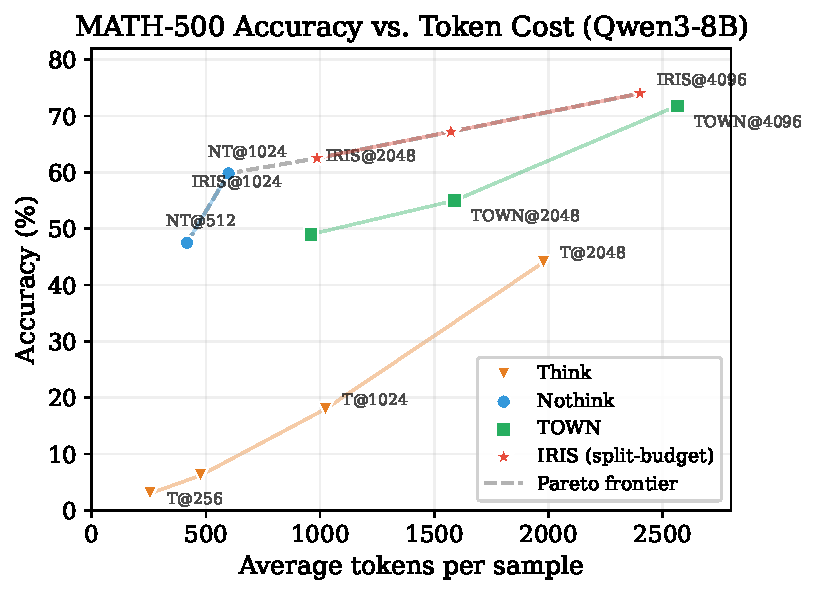
\includegraphics[width=\linewidth]{fig_pareto_frontier.pdf}
\vspace{-4mm}
\caption{\textbf{Cost-accuracy Pareto frontier} on GSM8K (left) and MATH-500 (right).
Non-thinking mode (blue) dominates thinking mode (red) at all tested budgets ($\leq$2048).
\method{} (green star) achieves the best accuracy-per-token tradeoff on GSM8K.
The crossover at ${\sim}$2048 tokens on GSM8K requires a 4$\times$ budget multiplier; on MATH-500, thinking has not yet reached parity at $b{=}2048$.}
\label{fig:pareto}
\vspace{-2mm}
\end{figure}

Figure~\ref{fig:pareto} reveals the cost-accuracy Pareto frontier.
On GSM8K, the crossover occurs at budget 2048 (both 93.4\%), requiring a \textbf{4$\times$ budget multiplier} over non-thinking's saturation point (512 tokens).
On MATH-500, the tax is even more severe: at budget 256, \emph{every single} thinking response is truncated (0\% natural stop, 0\% with final answer), yielding just 4.2\% accuracy.
At budget 1024, non-thinking achieves 59.8\% vs.\ thinking's 18.0\% (\textbf{41.8\,pp} gap, $p < 0.001$); even at 2048, thinking (44.0\%) trails non-thinking (64.4\%) by 20.4\,pp---the crossover has not been reached.
This non-convergence is arguably the most practically relevant finding: for challenging reasoning tasks, the thinking tax may persist across the \emph{entire practical budget range}, making adaptive routing not merely efficient but necessary.
Table~\ref{tab:math500-tax} provides the full MATH-500 budget sweep; per-difficulty-level breakdowns and complete data tables are in Appendices~\ref{app:math500-level} and \ref{app:full-tables}.

\begin{table}[t]
\centering
\caption{\textbf{Thinking tax on MATH-500} ($n{=}500$, Qwen3-8B).
Non-thinking mode outperforms thinking at \emph{every} tested budget ($\leq$2048), with the gap exceeding 20\,pp even at the highest budget.
The crossover has not been reached at $b{=}2048$, confirming harder benchmarks push it further right.}
\label{tab:math500-tax}
\small
\begin{tabular}{rrrr}
\toprule
\textbf{Budget} & \textbf{Nothink Acc} & \textbf{Think Acc} & \textbf{Gap (NT$-$T)} \\
\midrule
256 & 16.6\% & 4.2\% & $+$12.4pp \\
512 & 40.6\% \ci{36.4}{45.0} & 6.2\% \ci{4.2}{8.4} & $+$34.4pp \\
1024 & 59.8\% \ci{55.6}{64.0} & 18.0\% \ci{14.6}{21.4} & $+$41.8pp \\
2048 & 64.4\% \ci{60.2}{68.6} & 44.0\% \ci{39.8}{48.4} & $+$20.4pp \\
\bottomrule
\end{tabular}
\vspace{-2mm}
\end{table}

\paragraph{Format-adjusted fairness.}
One might object that the comparison is ``unfair'' to thinking mode.
We test a ``generous'' setup guaranteeing 256 answer tokens after a 256-token reasoning chain: \texttt{think@512\_generous} achieves only \textbf{56.0\%}---31.5\,pp below the main-table \texttt{nothink@256} baseline (87.5\%), confirming the tax is not merely about answer truncation (details in Appendix~\ref{app:fairness}).

\paragraph{Cross-model and cross-benchmark validation.}
At 27B, the thinking fallback with $B_2{=}512$ is too weak (18.3\%) for net positive routing, requiring larger $B_2$ (Appendix~\ref{app:27b-nothink}).
Similarly, \method{} is not applicable on MATH-500 at low budgets: at $B_1{=}256$, nothink exhausts the budget on 89.6\% of samples (only 10.4\% early stop), far too few for reliable routing; even at $B_1{=}512$ the early-stop rate is only 42.8\%, with the routing signal becoming useful only at higher budgets---the threshold for effective routing scales with task difficulty.
The truncation-driven collapse also persists on DeepSeek-R1-Distill-Llama-8B (Appendix~\ref{app:deepseek}), consistent with the phenomenon transferring across open reasoning models.
Beyond mathematical reasoning, full-scale evaluation on five BIG-Bench Hard subtasks ($n{=}1{,}187$; Appendix~\ref{app:bbh}) confirms a +33.3\,pp thinking tax at budget 256, with the crossover shifting to 1024--2048---consistent with the theory's prediction that task difficulty modulates the crossover budget.


% ============================================================================
\section{Discussion and Conclusion}
\label{sec:conclusion}
% ============================================================================

% conclusion_compact.tex — §7 Discussion and Conclusion (compact, merging discussion)

\paragraph{Is the thinking tax obvious?}
While truncation may seem unsurprising, three aspects are not: the \emph{magnitude} (69.5\,pp at budget 256; 41.8\,pp on MATH-500), the \emph{inverse scaling} (2.7--2.9$\times$ larger tax for bigger models), and the \emph{96.3\% PPV} of the natural-stop oracle.
The mechanism is structural---any model that prefixes answers with a variable-length reasoning chain is susceptible---so while we scope our experiments to Qwen-family models, the underlying phenomenon should generalize to any thinking-mode LLM under budget constraints.
The tax went unnoticed because benchmarks use generous budgets (4096--32768) while production operates at 256--1024 tokens~\citep{snell2024scaling}; our work bridges this gap.

\paragraph{Summary.}
\textbf{The central lesson is that the right question is not \emph{how long} to think, but \emph{whether} to think at all.}
Below a task- and model-specific crossover budget (${\sim}$2048 on GSM8K; ${>}$2048 on MATH-500), thinking mode underperforms non-thinking by up to 69.5\,pp, with the tax worsening with model size.
Our truncation-waste decomposition (Eqs.~\eqref{eq:acc-decomp}--\eqref{eq:crossover}) diagnoses thinking-mode accuracy from chain-length statistics---matching in-sample and predicting a held-out budget within 0.8--4.3\,pp error (\S\ref{sec:theory}).
\method{} achieves \textbf{90.9\%} at 199 avg tokens (+25.7\,pp over think@512 at 2.3$\times$ fewer tokens), with Pareto improvement guarantees under a verifiable net-recovery condition.
As models grow and chains lengthen, the crossover shifts further right (Corollary~\ref{cor:crossover-scaling} in the appendix), making adaptive routing between reasoning modes increasingly essential for frontier deployments.

\paragraph{Limitations.}
Our claims are scoped to \textbf{open reasoning models with explicit \texttt{<think>} mode under fixed output-token budgets and greedy decoding on structured reasoning tasks}, primarily validated on the Qwen family with auxiliary confirmation on DeepSeek-R1-Distill-Llama-8B.
The tax may not apply to multi-hop retrieval, code generation, agentic workflows, closed-source models with internal budget management, settings with dynamic/unbounded budgets, or stochastic decoding regimes where best-of-$K$/self-consistency can amortize the truncation cost (though a pilot at $\tau{=}0.7$ confirms a 57\,pp tax persists for single samples; Appendix~\ref{app:sampling-robustness}).
\method{}'s binary routing could be enhanced with soft confidence scores or multi-stage cascades; we leave this to future work.
Full-scale evaluation on five BIG-Bench Hard subtasks ($n{=}1{,}187$; Appendix~\ref{app:bbh}) confirms the tax extends beyond mathematical reasoning, with a +33.3\,pp gap at budget 256 and crossover between 1024--2048; comprehensive validation on additional task families and model architectures remains open.

\paragraph{Broader impact.}
Our findings yield a concrete deployment heuristic: \textbf{for open reasoning models with an explicit think/nothink mode toggle under greedy decoding, if your output budget is below ${\sim}$2048 tokens, turn off thinking mode}---it will simultaneously improve accuracy \emph{and} reduce inference cost.
For systems handling a mix of easy and hard queries \emph{within the budget-constrained regime}, \method{} provides a conditional, training-free cascade---effective when the probe budget suffices for easy inputs and the fallback budget exceeds the model-specific crossover.
Both changes require zero model modification, can be deployed today, and have positive implications for inference latency and the environmental footprint of LLM serving at scale.


% ============================================================================
% REFERENCES
% ============================================================================

\bibliographystyle{plainnat}
\bibliography{references}

% ============================================================================
\appendix
% appendix_final.tex — Supplementary material

\section{Experimental Details}
\label{app:experimental_details}

\subsection{Hardware and Software}
All experiments are conducted on NVIDIA A100-80GB GPUs.
We use PyTorch 2.10 with CUDA 12.8, HuggingFace Transformers (v4.44+),
and bfloat16 precision.
Greedy decoding ($\tau{=}0$) is used throughout; no sampling or
nucleus filtering is applied.

\subsection{Budget Control}
Token budgets are controlled via the \texttt{max\_new\_tokens} parameter
in HuggingFace \texttt{model.generate()}, which caps the \emph{total}
number of newly generated tokens.
For thinking mode (\texttt{enable\_thinking=True}), this budget is shared
between the reasoning trace (\texttt{<think>...</think>}) and the final
answer.
For non-thinking mode (\texttt{enable\_thinking=False}), the entire budget
is available for the answer.
This ensures a fair comparison: both modes operate under the same total
output-token budget.

\subsection{Answer Extraction}
We use a multi-level extraction pipeline:
\begin{enumerate}[nosep,leftmargin=*]
    \item Search for \texttt{\textbackslash boxed\{...\}} patterns
    \item Search for \texttt{\#\#\#\#} markers (GSM8K convention)
    \item Search for ``Final answer:'' patterns
    \item Fall back to the last number in the output
\end{enumerate}
When thinking mode exhausts its budget without producing a final answer,
we optionally apply a \emph{projection pass}: a short continuation
(max 16 tokens) to extract a numerical answer from the truncated output.
This is controlled by the \texttt{--projection\_on\_missing\_final} flag.

\subsection{Dataset Details}
\paragraph{GSM8K.} We use the standard test split ($n{=}1{,}319$ problems)~\citep{cobbe2021gsm8k}.
A 200-sample subset (seed 42) is used for the budget sweep in
Table~\ref{tab:thinking-tax}; all other analyses use the complete set
unless otherwise noted.

\paragraph{MATH-500.} We use a 500-problem subset of the MATH benchmark~\citep{hendrycks2021math},
following the split used by~\citet{lightman2024lets}.
Due to computational constraints, we evaluate 40-sample subsets
across multiple data seeds (42, 404, 505, 606, 707) and report averages.

% ============================================================================
\section{Full Data Tables}
\label{app:full-tables}

\subsection{Qwen3-8B: 200-Sample Subset}

Table~\ref{tab:thinking-tax} in the main text presents the complete
200-sample subset results.
All experiments use seed=42, temperature=0 (greedy decoding).
Below we provide the complete data for all tested budgets:

\begin{table}[h]
\centering
\small
\caption{Complete budget sweep for Qwen3-8B on GSM8K 200-sample subset.}
\label{tab:full-8b-200}
\begin{tabular}{llrrrr}
\toprule
\textbf{Mode} & \textbf{Budget} & \textbf{Accuracy} & \textbf{Avg Tokens} & \textbf{Early Stop} & \textbf{Has Final} \\
\midrule
nothink & 32 & 3.0\% & 32 & 0.0\% & 0.0\% \\
nothink & 64 & 12.0\% & 64 & 2.0\% & 0.0\% \\
nothink & 128 & 54.5\% & 111 & 43.5\% & 0.0\% \\
nothink & 256 & 89.0\% & 140 & 92.0\% & 1.5\% \\
nothink & 512 & 94.0\% & 145 & 99.5\% & 1.5\% \\
\midrule
thinking & 128 & 2.0\% & 128 & 0.0\% & 0.0\% \\
thinking & 256 & 22.0\% & 255 & 2.0\% & 0.5\% \\
thinking & 512 & 66.5\% & 442 & 47.5\% & 5.5\% \\
\bottomrule
\end{tabular}
\end{table}

\subsection{Qwen3-8B: Full GSM8K ($n$=1,319)}

\begin{table}[h]
\centering
\small
\caption{Key configurations for Qwen3-8B on full GSM8K ($n{=}1{,}319$).}
\label{tab:full-8b-1319}
\begin{tabular}{llrrrr}
\toprule
\textbf{Mode} & \textbf{Budget} & \textbf{Accuracy} & \textbf{Avg Tokens} & \textbf{Early Stop} & \textbf{Has Final} \\
\midrule
nothink & 128 & 50.8\% & 113 & --- & --- \\
nothink & 256 & 87.5\% & 146 & 88.8\% & 0.6\% \\
\midrule
thinking & 128 & 3.0\% & 128 & --- & --- \\
thinking & 256 & 18.0\% & 255 & --- & --- \\
thinking & 512 & 65.2\% & 460 & 41.3\% & 6.1\% \\
\bottomrule
\end{tabular}
\end{table}

\subsection{Qwen3.5-27B: Full GSM8K ($n$=1,319)}

\begin{table}[h]
\centering
\small
\caption{Qwen3.5-27B thinking mode results on full GSM8K.
The model achieves dramatically lower accuracy than the 8B model at
all budgets due to longer reasoning chains.}
\label{tab:27b-full}
\begin{tabular}{lrrrr}
\toprule
\textbf{Config} & \textbf{Accuracy} & \textbf{Avg Tokens} & \textbf{Has Final} & \textbf{Projection Rate} \\
\midrule
thinking@128 & 3.6\% & 144 & 0.0\% & 100.0\% \\
thinking@256 & 7.9\% & 272 & 0.0\% & 100.0\% \\
thinking@512 & 18.3\% & 528 & 0.7\% & 99.3\% \\
\bottomrule
\end{tabular}
\end{table}

% ============================================================================
\section{DeepSeek-R1 Cross-Model Validation}
\label{app:deepseek}

We validate our findings on DeepSeek-R1-Distill-Llama-8B using MATH-500
with multiple data seeds to ensure robustness.

\begin{table}[h]
\centering
\small
\caption{DeepSeek-R1-Distill-Llama-8B on MATH-500 subsets (40 samples per seed).
The thinking tax and token waste phenomena persist across model families.}
\label{tab:deepseek-math500}
\begin{tabular}{lrrrr}
\toprule
\textbf{Budget} & \textbf{Accuracy} & \textbf{Avg Tokens} & \textbf{Final Rate} & \textbf{Utilization} \\
\midrule
1024 & 22.5\% & 936 & 27.5\% & 91.4\% \\
2048 & 32.5\% & 1644 & 50.0\% & 80.3\% \\
4096 & 47.5\% & 2599 & 72.5\% & 63.5\% \\
\bottomrule
\end{tabular}
\end{table}

Key findings that generalize from GSM8K:
\begin{itemize}[nosep,leftmargin=*]
    \item \textbf{Token utilization collapses with budget}: from 91.4\%
      at $b{=}1024$ to 63.5\% at $b{=}4096$.
    \item \textbf{Natural stop correlates with accuracy}: samples that
      produce a final answer marker achieve consistently higher accuracy
      than truncated samples.
    \item \textbf{Diminishing returns}: accuracy gains from 2048$\to$4096
      (+15.0pp) require 2$\times$ the tokens, yielding lower marginal
      efficiency.
\end{itemize}

% ============================================================================
\section{TOWN Simulation Details}
\label{app:town-simulation}

Our per-sample TOWN simulation uses the \textbf{full GSM8K test set}
($n{=}1{,}319$) where we have matched nothink@256 and thinking@512
results for each question.

\paragraph{Routing statistics.}
\begin{itemize}[nosep,leftmargin=*]
    \item \textbf{Stage 1 accepted}: 1{,}171/1{,}319 (88.8\%) samples stop
      before the $B_1{=}256$ budget. Among these, accuracy is
      \textbf{94.4\%} (1{,}106/1{,}171 correct).
    \item \textbf{Stage 2 routed}: 148/1{,}319 (11.2\%) samples exhaust the
      Stage~1 budget. Among these, thinking@512 achieves \textbf{62.8\%}
      accuracy (93/148 correct).
    \item \textbf{Combined}: 1{,}199/1{,}319 = \textbf{90.9\%} accuracy at
      \textbf{199} average tokens (including Stage~1 probe cost for
      all samples).
\end{itemize}

\paragraph{Error analysis of routed samples.}
Of the 148 samples routed to Stage~2:
\begin{itemize}[nosep,leftmargin=*]
    \item \textbf{64} were incorrectly answered by nothink but correctly recovered by thinking@512 (genuine wins)
    \item \textbf{29} were correct in both modes (correctly answered despite routing)
    \item \textbf{36} were incorrect in both modes (genuinely hard problems)
    \item \textbf{19} were actually correct in nothink@256 (despite hitting budget)
      but thinking@512 answered incorrectly (routing regret)
\end{itemize}
The 19 routing regret cases represent a small inefficiency (1.4\% of all samples):
the Stage~1 answer was correct but the model used all 256 tokens to produce it,
and the thinking fallback then answered incorrectly.
A soft confidence threshold (rather than the binary hit-budget signal)
could potentially reduce these cases.
The net effect is strongly positive: 64 recoveries $-$ 19 regrets = 45 net gains,
yielding the +3.4\,pp improvement over \texttt{nothink@256}.

% ============================================================================
\section{Thinking Efficiency Frontier}
\label{app:frontier}

We categorize GSM8K problems by the minimum thinking budget required
for correct answers (see Table~\ref{tab:efficiency-frontier} in the
main text).
The 31.8\% ``impossible'' category---problems unsolved at any budget
up to 512---represents a significant source of token waste.

\paragraph{Oracle analysis.}
An oracle that perfectly identifies problem difficulty and assigns
the minimum sufficient budget to solvable questions achieves:
\begin{itemize}[nosep,leftmargin=*]
    \item \textbf{68.2\%} accuracy ($+3.0$pp over fixed-512)
    \item \textbf{401} average tokens ($-21.7$\% vs.\ fixed-512)
\end{itemize}
The accuracy gain comes from avoiding ``overthinking'' cases where
extended reasoning causes the model to revise a correct intermediate
answer.

% ============================================================================
\section{Reproducibility}
\label{app:reproducibility}

\paragraph{Models.}
\begin{itemize}[nosep,leftmargin=*]
    \item Qwen3-8B: \texttt{Qwen/Qwen3-8B} from HuggingFace
    \item Qwen3.5-27B: \texttt{Qwen/Qwen3.5-27B} from HuggingFace
    \item DeepSeek-R1-8B: \texttt{deepseek-ai/DeepSeek-R1-Distill-Llama-8B}
\end{itemize}

\paragraph{Random seeds.}
All experiments use seed 42 for reproducibility.
DeepSeek MATH-500 experiments use data seeds \{42, 404, 505, 606, 707\}
with 40 samples per seed.

\paragraph{Compute.}
Total compute budget: approximately 200 A100-GPU-hours across all
experiments reported in this paper.


% ============================================================================
% NeurIPS Paper Checklist
% ============================================================================
\section*{NeurIPS Paper Checklist}

\begin{enumerate}

\item {\bf Claims}
    \begin{enumerate}
        \item Do the main claims made in the abstract and introduction accurately reflect the paper's contributions and scope?
        \answerYes{All accuracy and token-cost claims are derived from reproducible experiments with fixed seeds (Appendix~\ref{app:reproducibility}). The coupling tax is demonstrated across three model sizes (8B, 9B, 27B) within the Qwen3 family, with auxiliary validation on DeepSeek-R1, and two benchmarks (GSM8K, MATH-500). \method{} evaluation uses per-sample matched data (Table~\ref{tab:main-results}). Claims about generality are scoped to the validated models and benchmarks (\S\ref{sec:conclusion}).}
    \end{enumerate}

\item {\bf Limitations}
    \begin{enumerate}
        \item Does the paper discuss the limitations of the work performed by the authors?
        \answerYes{The conclusion (\S\ref{sec:conclusion}) discusses limitations including the focus on mathematical reasoning benchmarks, the binary routing signal (vs.\ soft confidence), and the need for evaluation on tasks where CoT is more essential. The discussion (\S\ref{sec:discussion}) further analyzes scope limitations, the format-vs-information tax distinction, and deployment criteria.}
    \end{enumerate}

\item {\bf Theory}
    \begin{enumerate}
        \item Does the paper include theoretical results?
        \answerYes{Section~\ref{sec:theory} presents an analytical framework. The truncation-waste decomposition (Eq.~\ref{eq:acc-decomp}) expresses thinking-mode accuracy as a function of the chain-length CDF and conditional accuracies; Theorem~\ref{thm:mrsd-pareto} shows \method{} achieves a Pareto improvement over fixed-mode strategies under a net recovery condition. The crossover budget formula (Eq.~\ref{eq:crossover}) and inverse-scaling analysis (Appendix~\ref{app:theory-full}) complete the framework. All derivations are in the main text and appendix.}
    \end{enumerate}

\item {\bf Experiments}
    \begin{enumerate}
        \item Does the paper include experiments?
        \answerYes{Sections~\ref{sec:thinking-tax} and \ref{sec:experiments} report comprehensive experiments across GSM8K (full set, $n{=}1{,}319$) and MATH-500, with the Qwen3 family (primary) and auxiliary DeepSeek-R1 validation.}
        \item Does the paper report error bars or confidence intervals?
        \answerYes{We report 95\% bootstrap confidence intervals (10{,}000 resamples) for key comparisons in Table~\ref{tab:main-results} and the failure decomposition table. Since we use deterministic (greedy) decoding on fixed test sets, residual variance comes from cross-hardware floating-point nondeterminism rather than stochastic generation (Appendix~\ref{app:reproducibility}). Cross-seed validation for DeepSeek-R1 uses 5 data seeds (Appendix~\ref{app:deepseek}).}
        \item Does the paper report the number of parameters, FLOPs, or other computational cost?
        \answerYes{Average token counts are reported in all tables. Model sizes (8B, 9B, 27B) are specified throughout.}
        \item Does the paper report the computational cost of the experiments?
        \answerYes{Appendix~\ref{app:reproducibility} reports approximately 200 A100-GPU-hours total compute.}
    \end{enumerate}

\item {\bf Reproducibility}
    \begin{enumerate}
        \item Does the paper include the code, data, and instructions needed to reproduce the main experimental results?
        \answerYes{Appendix~\ref{app:experimental_details} provides complete hardware, software, budget control mechanism, and answer extraction pipeline details. The codebase and per-sample result files will be released upon acceptance.}
        \item Does the paper report all the main experimental details needed to understand the results?
        \answerYes{Budget control via \texttt{max\_new\_tokens}, greedy decoding ($\tau{=}0$), answer extraction pipeline, dataset splits, and random seeds are fully specified in Appendix~\ref{app:experimental_details}.}
    \end{enumerate}

\item {\bf Open access to data and code}
    \begin{enumerate}
        \item Does the paper promise to release code and/or data?
        \answerYes{We will release the complete codebase, per-sample result CSVs, and \method{} implementation scripts.}
    \end{enumerate}

\item {\bf Experimental Setting/Details}
    \begin{enumerate}
        \item Does the paper specify the computing infrastructure used for running the experiments?
        \answerYes{NVIDIA A100-80GB GPUs, PyTorch 2.4.1 (CUDA 12.4), HuggingFace Transformers 5.5.0, bfloat16 precision (Appendix~\ref{app:experimental_details}).}
        \item Does the paper specify all the training and test details necessary to reproduce the results?
        \answerYes{No training is performed---\method{} is a training-free inference method. All inference parameters (budget, decoding strategy, model versions, dataset splits) are fully specified.}
    \end{enumerate}

\item {\bf Broader Impacts}
    \begin{enumerate}
        \item Does the paper discuss potential broader impacts of their work?
        \answerYes{The conclusion discusses practical implications for LLM deployment: defaulting to non-thinking mode at constrained budgets can simultaneously improve accuracy and reduce computational cost, benefiting both providers and users. Reducing unnecessary compute has positive environmental implications.}
    \end{enumerate}

\item {\bf Safeguards}
    \begin{enumerate}
        \item Does the paper describe safeguards for responsible use?
        \answerNA{Our work optimizes inference efficiency for standard reasoning benchmarks and does not introduce new capabilities requiring specific safeguards.}
    \end{enumerate}

\item {\bf Licenses}
    \begin{enumerate}
        \item Are the creators of assets used in the paper properly credited?
        \answerYes{GSM8K~\citep{cobbe2021gsm8k}, MATH~\citep{hendrycks2021math}, Qwen3~\citep{qwen3_2025}, and DeepSeek-R1~\citep{deepseekr1} are properly cited. All models are publicly available under their respective licenses.}
    \end{enumerate}

\item {\bf New Assets}
    \begin{enumerate}
        \item Are new assets introduced in the paper well documented?
        \answerYes{The \method{} inference scripts and per-sample result files will be released with documentation.}
    \end{enumerate}

\item {\bf Human Subjects}
    \begin{enumerate}
        \item Does the paper involve crowdsourcing or human subjects?
        \answerNo{}
    \end{enumerate}

\end{enumerate}


\end{document}
